\section{Pythagorean Triples}

A \textbf{Primitive Pythagorean Triple (PPT)} is a tuple $(a, b, c)$ where $a$, $b$, $c$ have no common factors and satisfy $a^{2}+b^{2}=c^{2}$. It has few features:

\begin{observation}
One of $a$ \& $b$ is odd and the other even, so $c$ is always odd.
\end{observation}

\begin{observation}
If $(a, b, c)$ is PPT, then we can factor $a^{2}=c^{2}-b^{2}$. It looks like $c - b$ and $c + b$ are themselves always squares and have no common factors.
\end{observation}

\begin{proof}
I first prove that $gcd(c - b, c + b) = 1$. \\
Let $d = gcd(c - b, c + b)$. \\ 
Then $c - b = dk$, $c + b = dl$, $k,l\in \mathbb{N}$. \\
Since $2b = d(l - k)$ and $2c = d(l + k)$, $d\mid gcd(2b, 2c)$. \\
Now suppose $gcd(b, c)= g > 1$. \\
Set $b = g\tilde{b}$, $c = g\tilde{c}$. \\
Then $a^{2} = g^{2}(\tilde{c}^{2} - \tilde{b}^{2})$, which leads to $g\mid a$. \\
However, this is a contradiction by \textbf{Observation 2.1.1}. \\
Thus, $gcd(b, c) = 1$ and $gcd(2b, 2c) = 2$. \\
We now know that $d = 1$ or $d = 2$ as $d \mid gcd(2b, 2c)$. \\
If $d = 2$, then $a^{2}=(c-b)(c+b)=4kl$ so $2\mid a$, which is again a contradiction. \\
Thus $d = 1$.\\
\\
Now I prove $c - b$ and $c + b$ are squares. \\
Let $a = p_{1}^{n_{1}}\dots p_{r}^{n_{r}}$ where $p_{i}$ prime, $n\in \mathbb{N}$. \\
Then $a^{2} = p_{1}^{2n_{1}}\dots p_{r}^{2n_{r}} = (c - b)(c + b)$. \\ 
As $gcd(c - b, c + b) = 1$ by \textbf{Observation 2.1.1}, they are squares.
\end{proof}

\noindent
A \textbf{Primitive Pythagorean Pair (PPP)} is a pair $(s, t)$ s.t. $a = st$, $b = \dfrac{s^{2} - t^{2}}{2}$, $c = \dfrac{s^{2} + t^{2}}{2}$. \\
We can induce it by substituting $c + b = s^{2}$, $c - b = t^{2}$. \\
\\
It is worth noting the relationship between the PPT and unit circle. We start by dividing the both sides of $a^{2} + b^{2} = c^{2}$ by $c^{2}$. Then we can induce the typical unit circle form by substituting as $x = \dfrac{a}{c}$ and $y = \dfrac{b}{c}$. Our goal is to find $(x, y)$ where $x, y\in \mathbb{Q}$.

\begin{figure}[h]
\caption{A Unit Circle and a line passing through (-1, 0)}
\centering
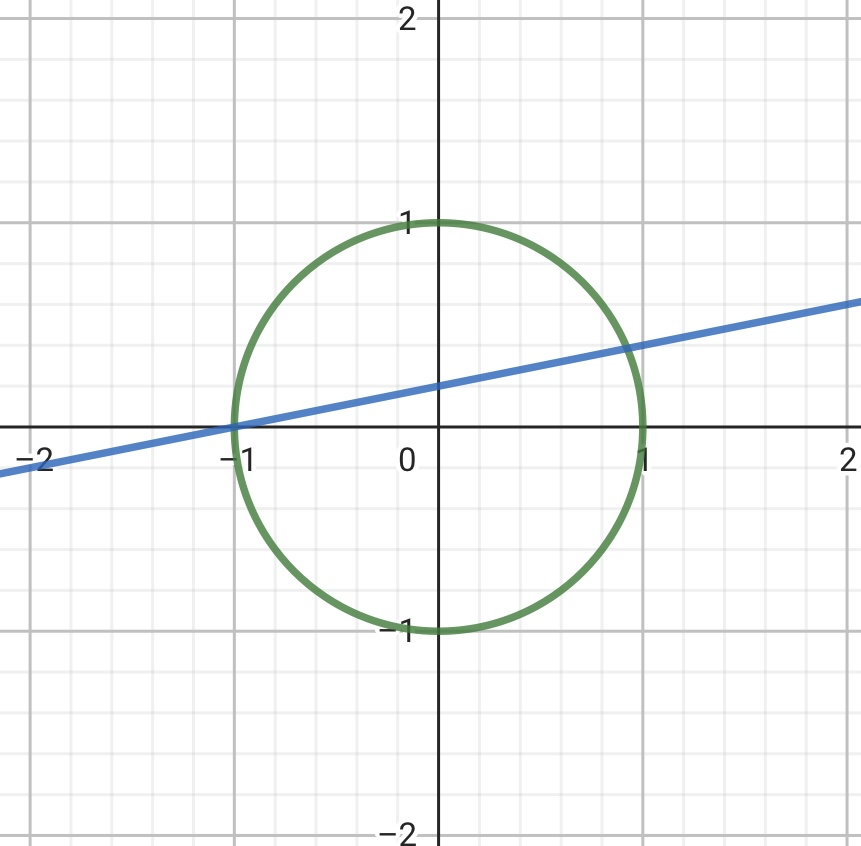
\includegraphics[width=0.5\textwidth]{number_theory/fig2-1.jpg}
\end{figure}

We find by exploiting geometry. As we know the trivial solution $(-1, 0)$, we draw a line that passes through $(-1, 0)$ and get the coordinate of the intersection other than $(-1, 0)$. We set the slope of the line $m\in \mathbb{Q}$ so that all the intersections are of $\mathbb{Q}\times \mathbb{Q}$. 
\begin{align*}
x^{2} + m^{2}(x + 1)^{2} &= 1
(1 + m^{2})x^{2} + 2m^{2}x + (m^{2} - 1) &= 0
(x, y) &= (\frac{1 - m^{2}}{1 + m^{2}}, \frac{2m}{1 + m^{2}})
\end{align*}

Now let $m = \dfrac{v}{u}$ as $m\in \mathbb{Q}$. Then we can finally induce another way to describe Pythagorean triples: $(a, b, c) = (u^{2} - v^{2}, 2uv, u^{2} + v^{2})$. This is equivalent form when $u = \dfrac{s + t}{2}$, $v = \dfrac{s - t}{2}$. Note that not all $u$, $v$ give us PPT.